% Generated by extension/generality/make_assets.py. Do not edit.
\definecolor{propcol}{HTML}{217D91}
\definecolor{pairedcol}{HTML}{5D6670}
\definecolor{semicol}{HTML}{C9803A}
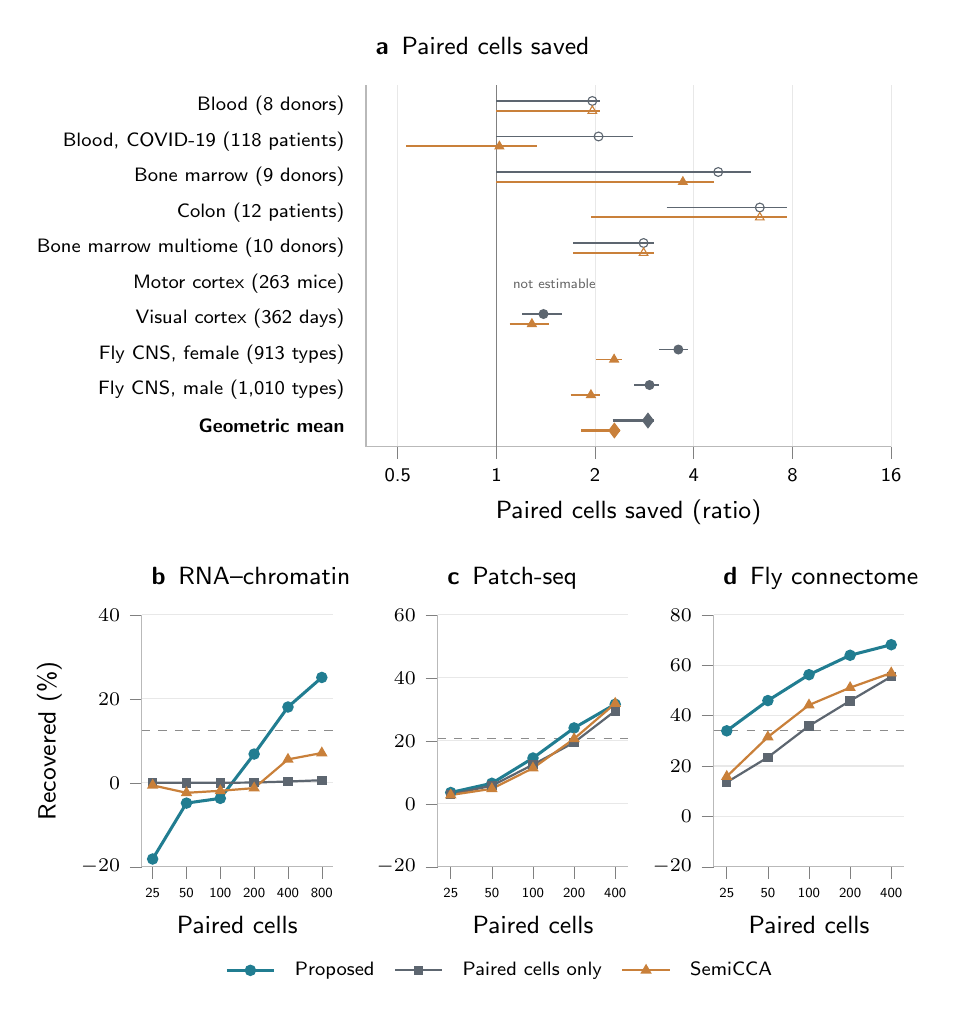
\begin{tikzpicture}[font=\sffamily]
\begin{axis}[name=a,scale only axis,width=.55\textwidth,height=4.6cm,xmode=log,log basis x=2,
 xmin=0.4,xmax=16,ymin=-.6,ymax=9.6,xtick={0.5,1,2,4,8,16},xticklabels={0.5,1,2,4,8,16},
 ytick={0,1,2,3,4,5,6,7,8,9},
 yticklabels={{\textbf{Geometric mean}},{Fly CNS, male (1,010 types)},{Fly CNS, female (913 types)},{Visual cortex (362 days)},{Motor cortex (263 mice)},{Bone marrow multiome (10 donors)},{Colon (12 patients)},{Bone marrow (9 donors)},{Blood, COVID-19 (118 patients)},{Blood (8 donors)}},
 xlabel={Paired cells saved (ratio)},
 title={\textbf{a}\enspace Paired cells saved},
 axis x line*=bottom,axis y line*=left,tick align=outside,xmajorgrids=true,grid style={gray!18},axis line style={gray!55},tick label style={font=\sffamily\scriptsize},label style={font=\sffamily\small},clip=false,title style={font=\sffamily\small,at={(0,1)},anchor=base west,yshift=5pt},y tick style={draw=none},yticklabel style={font=\sffamily\scriptsize}]
\draw[black!50] (axis cs:1,-.6) -- (axis cs:1,9.6);
\draw[color=pairedcol,line width=.7pt] (axis cs:2.631,1.14) -- (axis cs:3.133,1.14);
\addplot[only marks,color=pairedcol,mark=*,mark size=1.6pt] coordinates { (2.932,1.14) };
\draw[color=pairedcol,line width=.7pt] (axis cs:3.144,2.14) -- (axis cs:3.849,2.14);
\addplot[only marks,color=pairedcol,mark=*,mark size=1.6pt] coordinates { (3.590,2.14) };
\draw[color=pairedcol,line width=.7pt] (axis cs:1.198,3.14) -- (axis cs:1.587,3.14);
\addplot[only marks,color=pairedcol,mark=*,mark size=1.6pt] coordinates { (1.392,3.14) };
\node[font=\sffamily\tiny,color=black!60,anchor=west] at (axis cs:1.05,4.00) {not estimable};
\draw[color=pairedcol,line width=.7pt] (axis cs:1.713,5.14) -- (axis cs:3.019,5.14);
\addplot[only marks,color=pairedcol,mark=o,mark size=1.6pt] coordinates { (2.812,5.14) };
\draw[color=pairedcol,line width=.7pt] (axis cs:3.304,6.14) -- (axis cs:7.701,6.14);
\addplot[only marks,color=pairedcol,mark=o,mark size=1.6pt] coordinates { (6.361,6.14) };
\draw[color=pairedcol,line width=.7pt] (axis cs:1.000,7.14) -- (axis cs:5.988,7.14);
\addplot[only marks,color=pairedcol,mark=o,mark size=1.6pt] coordinates { (4.750,7.14) };
\draw[color=pairedcol,line width=.7pt] (axis cs:1.000,8.14) -- (axis cs:2.604,8.14);
\addplot[only marks,color=pairedcol,mark=o,mark size=1.6pt] coordinates { (2.049,8.14) };
\draw[color=pairedcol,line width=.7pt] (axis cs:1.000,9.14) -- (axis cs:2.075,9.14);
\addplot[only marks,color=pairedcol,mark=o,mark size=1.6pt] coordinates { (1.962,9.14) };
\draw[color=pairedcol,line width=1pt] (axis cs:2.263,0.14) -- (axis cs:3.029,0.14);
\addplot[only marks,color=pairedcol,mark=diamond*,mark size=2.6pt] coordinates { (2.900,0.14) };
\draw[color=semicol,line width=.7pt] (axis cs:1.683,0.86) -- (axis cs:2.068,0.86);
\addplot[only marks,color=semicol,mark=triangle*,mark size=1.8pt] coordinates { (1.943,0.86) };
\draw[color=semicol,line width=.7pt] (axis cs:2.017,1.86) -- (axis cs:2.417,1.86);
\addplot[only marks,color=semicol,mark=triangle*,mark size=1.8pt] coordinates { (2.286,1.86) };
\draw[color=semicol,line width=.7pt] (axis cs:1.097,2.86) -- (axis cs:1.451,2.86);
\addplot[only marks,color=semicol,mark=triangle*,mark size=1.8pt] coordinates { (1.283,2.86) };
\draw[color=semicol,line width=.7pt] (axis cs:1.713,4.86) -- (axis cs:3.019,4.86);
\addplot[only marks,color=semicol,mark=triangle,mark size=1.8pt] coordinates { (2.812,4.86) };
\draw[color=semicol,line width=.7pt] (axis cs:1.946,5.86) -- (axis cs:7.701,5.86);
\addplot[only marks,color=semicol,mark=triangle,mark size=1.8pt] coordinates { (6.361,5.86) };
\draw[color=semicol,line width=.7pt] (axis cs:1.000,6.86) -- (axis cs:4.619,6.86);
\addplot[only marks,color=semicol,mark=triangle*,mark size=1.8pt] coordinates { (3.706,6.86) };
\draw[color=semicol,line width=.7pt] (axis cs:0.530,7.86) -- (axis cs:1.330,7.86);
\addplot[only marks,color=semicol,mark=triangle*,mark size=1.8pt] coordinates { (1.021,7.86) };
\draw[color=semicol,line width=.7pt] (axis cs:1.000,8.86) -- (axis cs:2.075,8.86);
\addplot[only marks,color=semicol,mark=triangle,mark size=1.8pt] coordinates { (1.962,8.86) };
\draw[color=semicol,line width=1pt] (axis cs:1.816,-0.14) -- (axis cs:2.383,-0.14);
\addplot[only marks,color=semicol,mark=diamond*,mark size=2.6pt] coordinates { (2.290,-0.14) };
\end{axis}
\begin{axis}[at={(a.outer south west)},anchor=outer north west,yshift=-.3cm,name=b,scale only axis,width=.2\textwidth,height=3.2cm,xmode=log,log basis x=2,
 xmin=20.0,xmax=1000.0,ymin=-20,ymax=40,xtick={25,50,100,200,400,800},xticklabels={25,50,100,200,400,800},
 xlabel={Paired cells},ylabel={Recovered (\%)},
 x tick label style={font=\sffamily\tiny},
 title={\textbf{b}\enspace RNA--chromatin},
 axis x line*=bottom,axis y line*=left,tick align=outside,ymajorgrids=true,grid style={gray!18},axis line style={gray!55},tick label style={font=\sffamily\scriptsize},label style={font=\sffamily\small},clip=false,title style={font=\sffamily\small,at={(0,1)},anchor=base west,yshift=5pt}]
\draw[dashed,black!45] (axis cs:20.0,12.5) -- (axis cs:1000.0,12.5);
\addplot[color=propcol,line width=1.1pt,mark=*,mark size=1.5pt] coordinates { (25,-18.14) (50,-4.83) (100,-3.70) (200,6.85) (400,18.05) (800,25.09) };
\addplot[color=pairedcol,line width=.8pt,mark=square*,mark size=1.3pt] coordinates { (25,0.00) (50,0.00) (100,0.00) (200,0.07) (400,0.31) (800,0.62) };
\addplot[color=semicol,line width=.8pt,mark=triangle*,mark size=1.6pt] coordinates { (25,-0.60) (50,-2.38) (100,-1.90) (200,-1.26) (400,5.58) (800,7.10) };
\end{axis}
\begin{axis}[at={(b.outer north east)},anchor=outer north west,xshift=.1cm,name=c,scale only axis,width=.2\textwidth,height=3.2cm,xmode=log,log basis x=2,
 xmin=20.0,xmax=500.0,ymin=-20,ymax=60,xtick={25,50,100,200,400},xticklabels={25,50,100,200,400},
 xlabel={Paired cells},
 x tick label style={font=\sffamily\tiny},
 title={\textbf{c}\enspace Patch-seq},
 axis x line*=bottom,axis y line*=left,tick align=outside,ymajorgrids=true,grid style={gray!18},axis line style={gray!55},tick label style={font=\sffamily\scriptsize},label style={font=\sffamily\small},clip=false,title style={font=\sffamily\small,at={(0,1)},anchor=base west,yshift=5pt}]
\draw[dashed,black!45] (axis cs:20.0,20.8) -- (axis cs:500.0,20.8);
\addplot[color=propcol,line width=1.1pt,mark=*,mark size=1.5pt] coordinates { (25,3.59) (50,6.52) (100,14.54) (200,24.09) (400,31.63) };
\addplot[color=pairedcol,line width=.8pt,mark=square*,mark size=1.3pt] coordinates { (25,3.04) (50,5.74) (100,12.43) (200,19.48) (400,29.50) };
\addplot[color=semicol,line width=.8pt,mark=triangle*,mark size=1.6pt] coordinates { (25,2.80) (50,4.77) (100,11.34) (200,20.64) (400,31.87) };
\end{axis}
\begin{axis}[at={(c.outer north east)},anchor=outer north west,xshift=.1cm,name=d,scale only axis,width=.2\textwidth,height=3.2cm,xmode=log,log basis x=2,
 xmin=20.0,xmax=500.0,ymin=-20,ymax=80,xtick={25,50,100,200,400},xticklabels={25,50,100,200,400},
 xlabel={Paired cells},
 x tick label style={font=\sffamily\tiny},
 title={\textbf{d}\enspace Fly connectome},
 axis x line*=bottom,axis y line*=left,tick align=outside,ymajorgrids=true,grid style={gray!18},axis line style={gray!55},tick label style={font=\sffamily\scriptsize},label style={font=\sffamily\small},clip=false,title style={font=\sffamily\small,at={(0,1)},anchor=base west,yshift=5pt}]
\draw[dashed,black!45] (axis cs:20.0,34.1) -- (axis cs:500.0,34.1);
\addplot[color=propcol,line width=1.1pt,mark=*,mark size=1.5pt] coordinates { (25,33.97) (50,45.97) (100,56.24) (200,63.95) (400,68.14) };
\addplot[color=pairedcol,line width=.8pt,mark=square*,mark size=1.3pt] coordinates { (25,13.53) (50,23.45) (100,35.91) (200,45.87) (400,55.47) };
\addplot[color=semicol,line width=.8pt,mark=triangle*,mark size=1.6pt] coordinates { (25,15.84) (50,31.52) (100,44.20) (200,51.10) (400,56.92) };
\end{axis}
\begin{axis}[hide axis,scale only axis,width=1pt,height=1pt,xmin=0,xmax=1,ymin=0,ymax=1,at={(c.outer south)},anchor=north,yshift=-2pt,legend style={draw=none,font=\sffamily\scriptsize,at={(0.5,0.5)},anchor=north,legend columns=3,column sep=5pt,cells={anchor=west}}]
\addlegendimage{color=propcol,line width=1.1pt,mark=*,mark size=1.5pt}
\addlegendentry{Proposed}
\addlegendimage{color=pairedcol,line width=.8pt,mark=square*,mark size=1.3pt}
\addlegendentry{Paired cells only}
\addlegendimage{color=semicol,line width=.8pt,mark=triangle*,mark size=1.6pt}
\addlegendentry{SemiCCA}
\end{axis}
\end{tikzpicture}
